\documentclass[18pt, aspectratio=169]{beamer}
\usepackage[utf8]{inputenc}
\usepackage{templates/beamerthemekit}
\usepackage{graphicx}
\usepackage{microtype}
\usepackage{xcolor}
\usepackage{hyperref}
\usepackage{multicol}
\usepackage{siunitx}
\usepackage{physics}
\usepackage{appendixnumberbeamer}
\usepackage{booktabs}
\usepackage{longtable}
\usepackage{listings}

\hypersetup{colorlinks, linkcolor=black, urlcolor=kit-blue100}

\lstset{
  basicstyle=\ttfamily,
  basicstyle=\footnotesize,
  language=C++,
}

\newcommand\pro{\item[$\oplus$]}
\newcommand\con{\item[$\ominus$]}

\newcommand{\greenbold}[1]{\textcolor{kit-green100}{\bf{#1}}}
\newcommand{\orangebold}[1]{\textcolor{kit-orange100}{\bf{#1}}}
\newcommand{\redbold}[1]{\textcolor{kit-red100}{\bf{#1}}}

\title{Track Quality Estimation for (Local) CDC Tracking}
\subtitle{From making CA tracking usable to a full CDC quality indicator}
\author{Michael Eliachevitch}
\date{14 May 2018}
\titleimage{tracks_wide}
\institute{ETP - KIT}

\begin{document}
\selectlanguage{english}

\begin{frame}
  \titlepage
\end{frame}

\begin{frame}
  \frametitle{Track Finding in the CDC}
  \begin{itemize}
  \item Legendre Algorithm:
    \begin{itemize}
    \item \greenbold{global} algorithm, transformation of all hits
    \item current CDC workhorse, works very well
    \item fast and stable against high backgrounds
    \item depends on assumptions: circular tracks through IP
    \end{itemize}
    \item Cellular Automaton (CA):
      \begin{itemize}
      \item developed by Oliver Frost
      \item use \greenbold{local relations} between nodes to build tracks
      \item less dependent on assumptions of track shape
      \item suffers from \greenbold{combinatorics}
      \item current use: \greenbold{finds segments} and attach them to Legendre tracks\\
        $\rightarrow$ \orangebold{increase hit efficiency}
      \end{itemize}
  \end{itemize}
\end{frame}

\begin{frame}
  \frametitle{CA track finding in the CDC}
  \begin{itemize}
  \item possible to use \greenbold{CA track finding} to \orangebold{increase finding efficiency}
    \begin{itemize}
    \item \greenbold{after global} track finding, run CA on remaining segment pairs
    \item promote single segments from 1st superlayer (curlers) to full tracks
    \item tracks from relations of axial + stereo segment pairs
    \item implemented, turn on with \lstinline[language=python]{add_cdc_track_finding(with_CA=True)}            
    \end{itemize}
    
  % \item solution: reject bad tracks \kitgreen{multivariate quality estimator}
  \end{itemize}
  \pause
  \begin{alertblock}{Problem: increased clone and fake rate}
    \begin{itemize}
    \item curling tracks found multiple times $\rightarrow$ clones
    \item short tracks from combinatorics $\rightarrow$ fakes and clones
    \end{itemize}
  \end{alertblock}

  \begin{block}{Solution: train a multivariate track classifier}
    \begin{itemize}
    \item reject bad tracks from CA\\
      $\rightarrow$ make CA tracking usable
    \item next step: use as input for  CDC quality indicator\\
    $\rightarrow$ full quality indicator wanted for analysis
    (\href{https://kds.kek.jp/indico/event/26522/session/10/contribution/75/material/slides/0.pdf}{overview
      talk})
  \item 
  

    
\end{itemize}
  \end{block}
\end{frame}

\begin{frame}
  \frametitle{Training the classifier}
  \begin{itemize}
  \item original idea: use MVA classifier to \greenbold{reject clones}
  \item based on existing MVA fake-rejection for Legendre tracks (using FastBDT)\\
    $\rightarrow$ truth target does not distinguish between clones
  \item idea: design truth target which knows clones
  \end{itemize}
  \begin{block}{``best match'' among clones}
    \begin{itemize}
    \item lowest \textbf{loop number}
    \item if equal, track with highest number of \textbf{matched hits}
    \end{itemize}
  \end{block}
  \begin{itemize}
  \item training with \texttt{FastBDT}, at the moment only track-wise features
  \item side effect: due to selection based on matched hits, also \greenbold{rejects fakes} from CA
  \end{itemize}
\end{frame}

\begin{frame}
  \frametitle{Results with CDC-only tracking}
  \begin{columns}
    \begin{column}{0.5\textwidth}
      \centering
      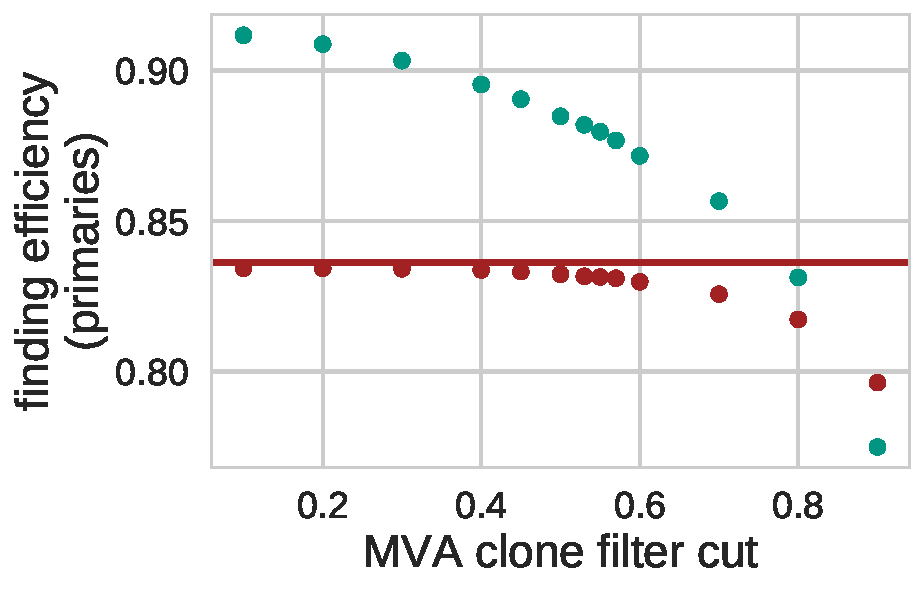
\includegraphics[width=1.0\textwidth]{figures/ca_is_matched_primaries.pdf}\\
      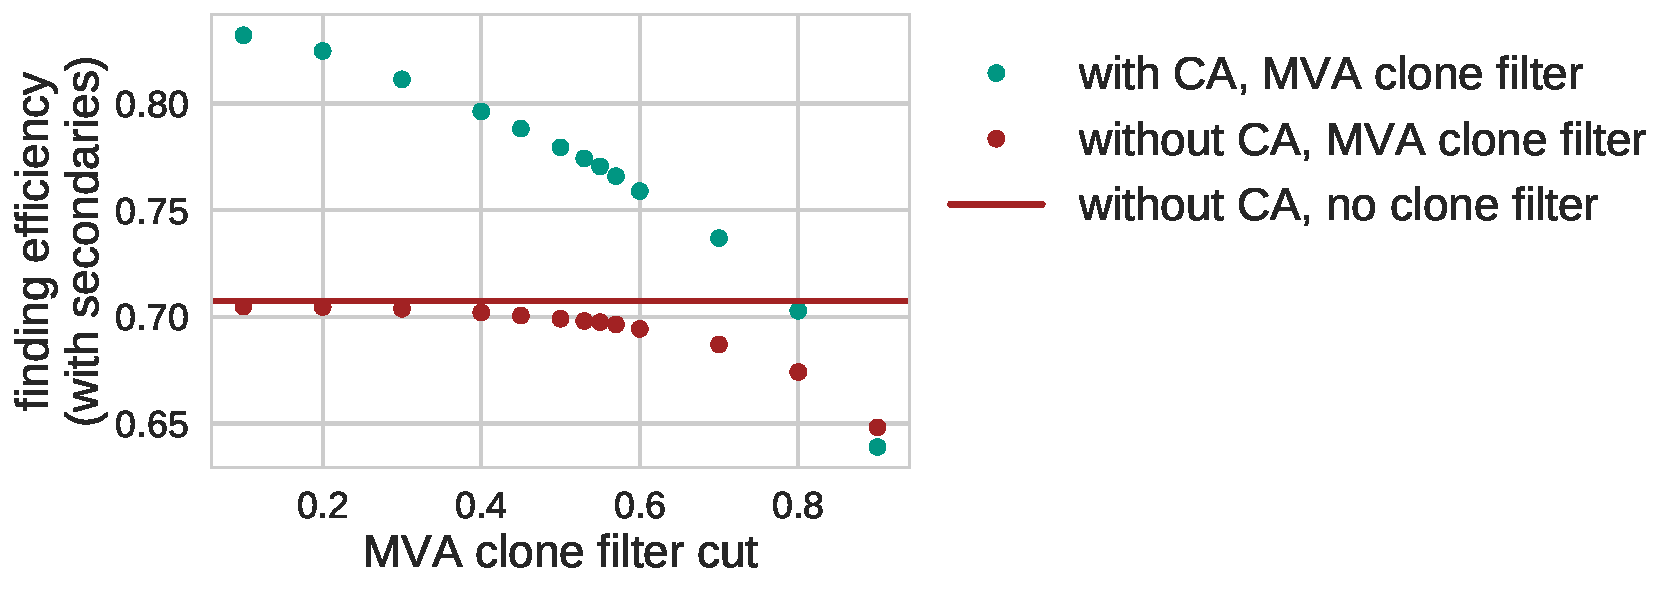
\includegraphics[width=1.0\textwidth]{figures/ca_is_matched_with_secondaries.pdf}
    \end{column}
    \begin{column}{0.5\textwidth}
      \centering
      \includegraphics[width=1.0\textwidth]{figures/ca_clone_rate.pdf}\\
      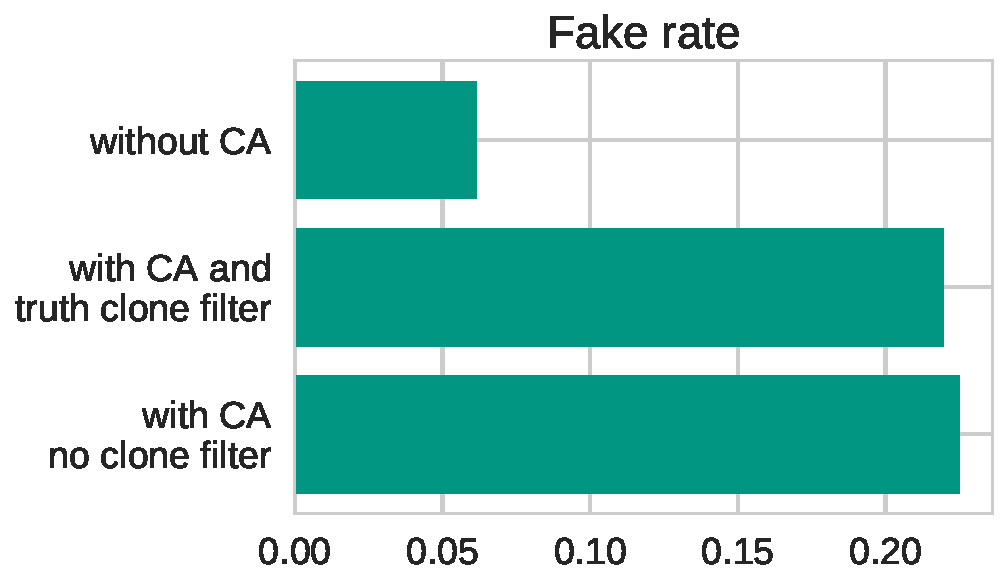
\includegraphics[width=1.0\textwidth]{figures/ca_fake_rate.pdf}
    \end{column}
  \end{columns}
  with cut around 0.5:
  \begin{itemize}
  \item finding efficiency with added CA higher than without CA
  \item fake and clone rate lower than in existing CDC-only tracking
  \end{itemize}
\end{frame}

\begin{frame}
  \frametitle{Results on full tracking,  including VXDTF2 + Kalman}
  \begin{columns}
    \begin{column}{0.5\textwidth}
      \centering
      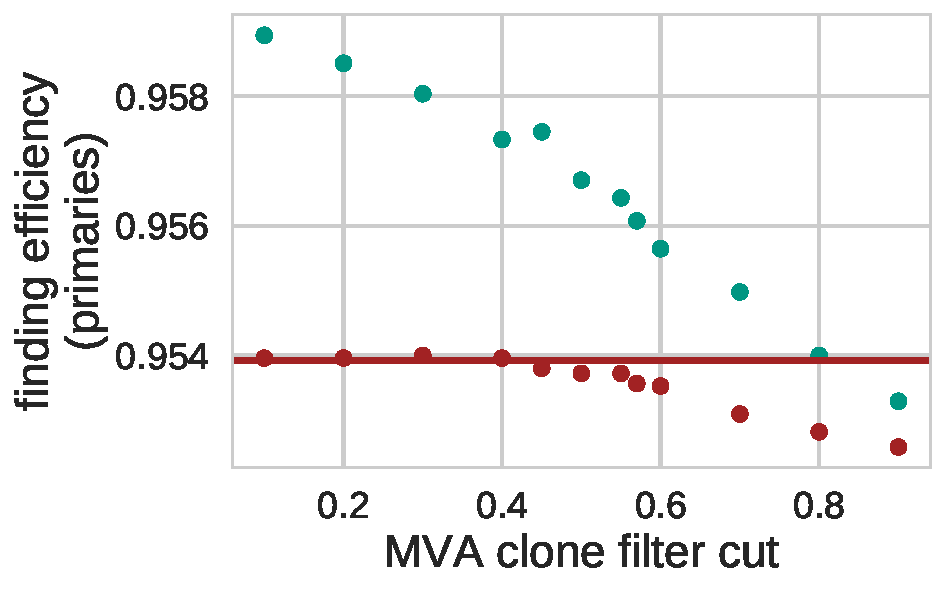
\includegraphics[width=1.0\textwidth]{figures/ca_is_matched_primaries_fullreco.pdf}\\
      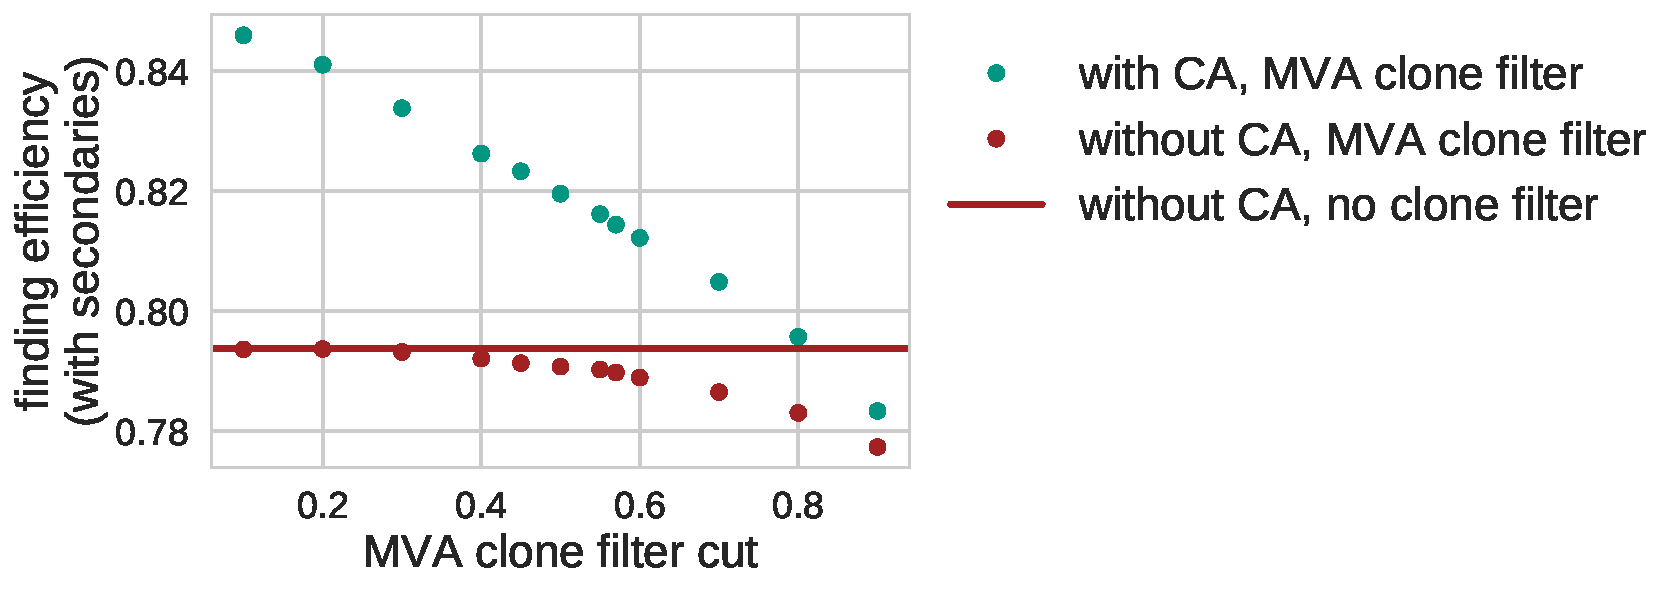
\includegraphics[width=1.0\textwidth]{figures/ca_is_matched_with_secondaries_fullreco.pdf}
    \end{column}
    \begin{column}{0.5\textwidth}
      \centering
      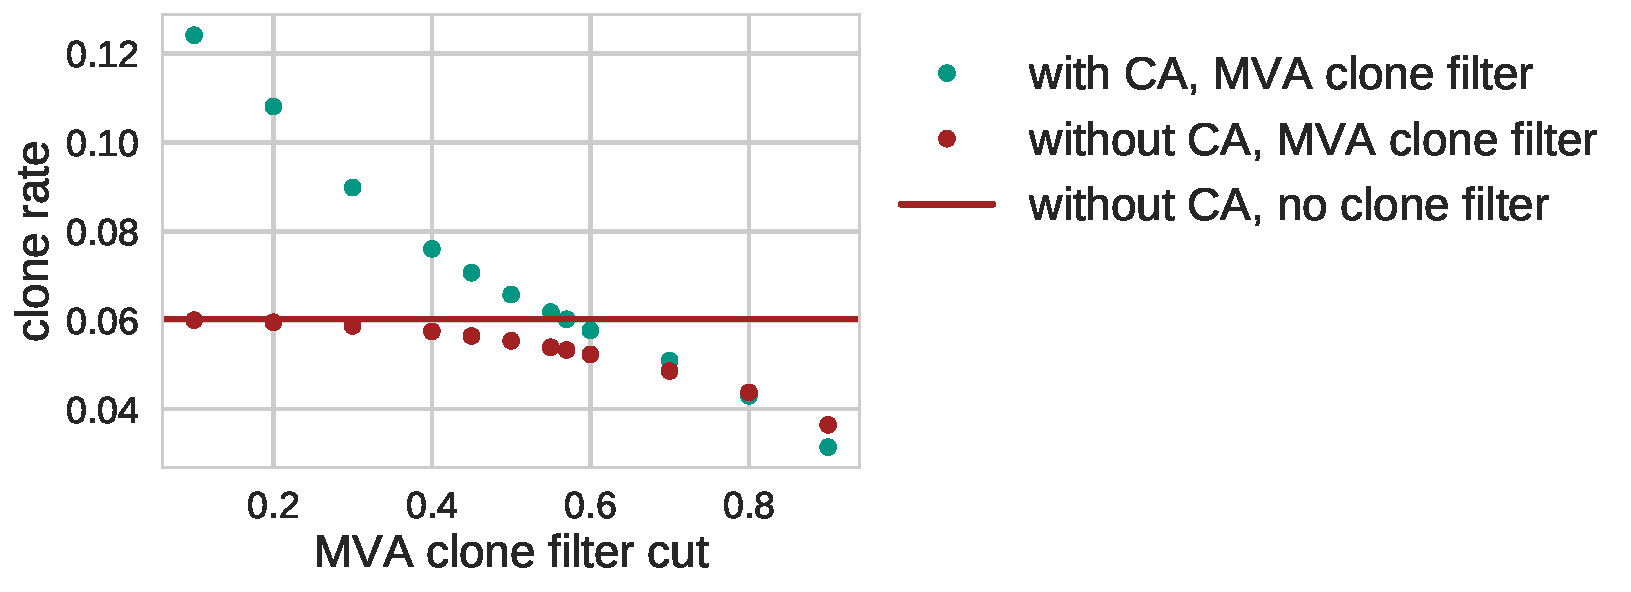
\includegraphics[width=1.0\textwidth]{figures/ca_clone_rate_fullreco.pdf}\\
      \includegraphics[width=1.0\textwidth]{figures/ca_fake_rate_fullreco.pdf}
    \end{column}
  \end{columns}
  \begin{itemize}
  \item finding efficiency on primaries changes $< \SI{0.5}{\percent}$\\
    low-$p_T$ tracks found by VXDTF2
  \item still large increase ($\sim$ \SI{2}{\percent}) with secondaries
  \end{itemize}
\end{frame}

\begin{frame}
  \frametitle{Hit efficiency in full tracking}
  \begin{columns}
    \begin{column}{0.7\textwidth}
      \centering
      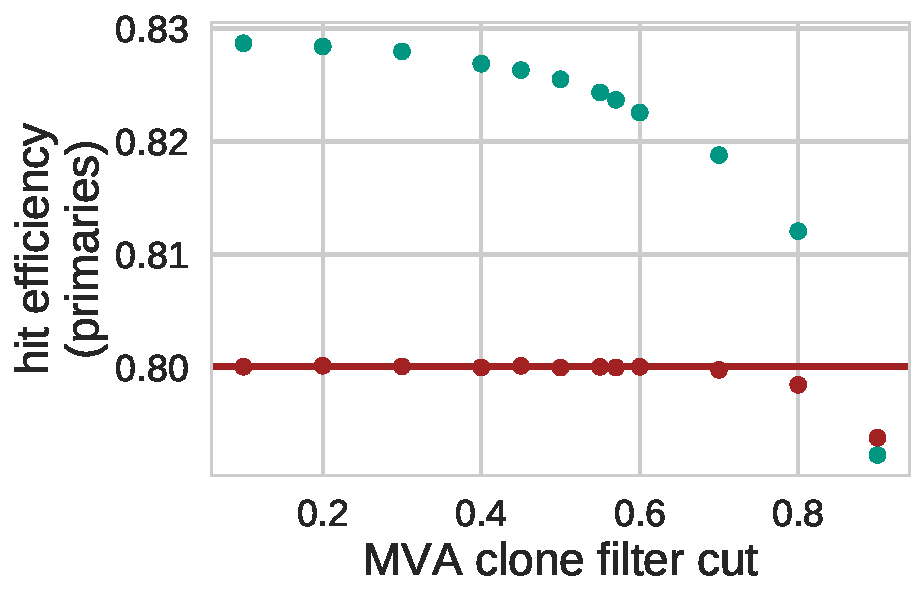
\includegraphics[width=1.0\textwidth]{figures/ca_hit_efficiency_primaries_fullreco.pdf}\\
    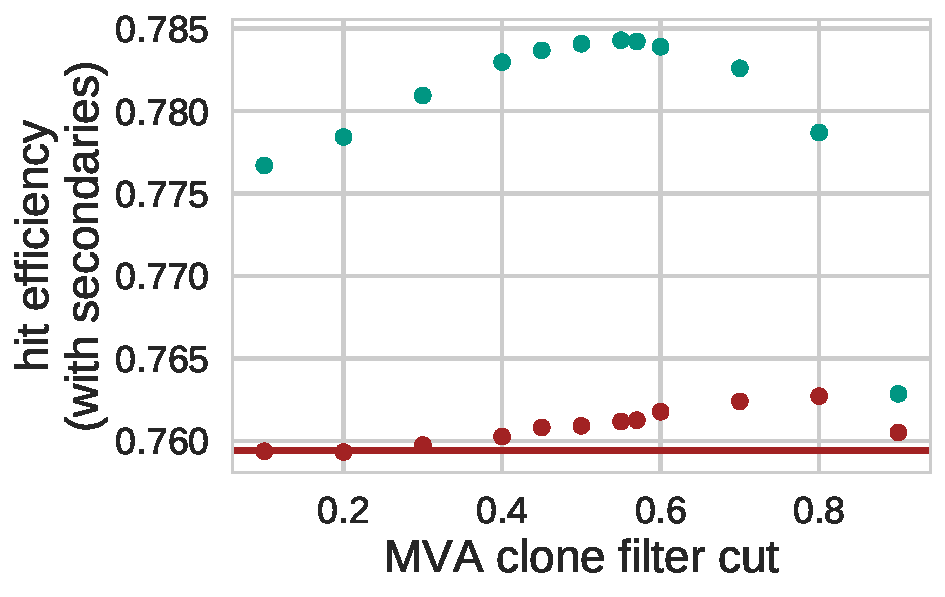
\includegraphics[width=1.0\textwidth]{figures/ca_hit_efficiency_with_secondaries_fullreco.pdf}\\
\end{column}
    \begin{column}{0.3\textwidth}
      \begin{itemize}
      \item \SI{2}{\percent}--\SI{3}{\percent} increase in hit efficiency
      \end{itemize}

    \end{column}
  \end{columns}
\end{frame}

\begin{frame}
  \frametitle{Track distributions}
  \begin{block}{Question}
    \begin{itemize}
    \item Classifier bias against interesting but rare tracks, e.g. with large impact parameters?
    \item In which parameter regions are the added/rejected tracks?
    \end{itemize}
  \end{block}
  \begin{columns}
    \begin{column}{.5\textwidth}
      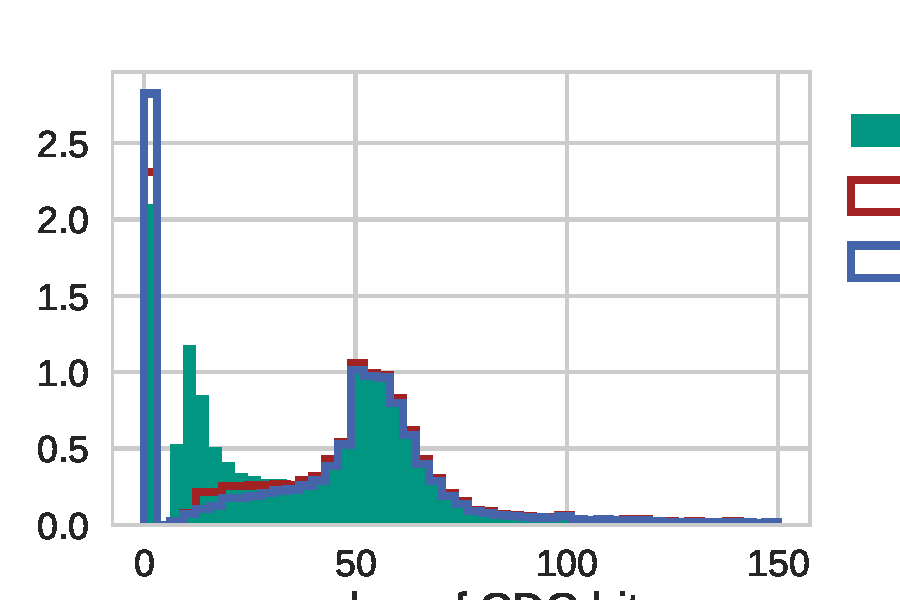
\includegraphics[width=1.0\textwidth]{figures/rejected_vs_other_track_distributions_by_found_n_cdc_hits_normed=False_scaleByEvents=True_fullreco.pdf}
    \end{column}
    \begin{column}{.5\textwidth}
      \includegraphics[width=1.0\textwidth]{figures/findeff_secondaries_by_d0_truth_fullreco.pdf}
    \end{column}
  \end{columns}  
\end{frame}

\begin{frame}
  \frametitle{Summary and outlook}
  \begin{itemize}
  \item design the training target, to accurately reflect intentions
  \item use event-wise features for clone-rejecting classifier
  \item \greenbold{store quality} indicator in reco tracks from CDC
  \end{itemize}
\end{frame}

\appendix
\backupbegin
\begin{frame}
  \centering \huge
  Backup
\end{frame}

\begin{frame}
  \frametitle{Features  used for CDC Track Rejecter training}
  As defined in \texttt{tracking/trackFindingCDC/filters/track/BasicTrackVarSet.h}
  \begin{columns}
    \begin{column}{0.5\textwidth}
      \begin{itemize}
      \item \lstinline{size}
      \item \lstinline{pt}
      \item \lstinline{sz_slope}
      \item \lstinline{drift_length_mean}
      \item \lstinline{drift_length_variance}
      \item \lstinline{drift_length_max}
      \item \lstinline{drift_length_min}
      \item \lstinline{drift_length_sum}
      \item \lstinline{adc_mean}
      \item \lstinline{adc_variance}
      \end{itemize}
    \end{column}
    \begin{column}{0.5\textwidth}
      \begin{itemize}

      \item \lstinline{adc_max}
      \item \lstinline{adc_min}
      \item \lstinline{adc_sum}
      \item \lstinline{empty_s_mean}
      \item \lstinline{empty_s_variance}
      \item \lstinline{empty_s_max}
      \item \lstinline{empty_s_min}
      \item \lstinline{empty_s_sum}
      \item \lstinline{has_matching_segment}
      \item \lstinline{s_range}
      \end{itemize}      
    \end{column}
  \end{columns}
\end{frame}

\begin{frame}[allowframebreaks]
  \frametitle{Plots from recording filter outputt}
  \includegraphics[width=0.4\textwidth]{figures/clone_multiplicities.pdf}\\
  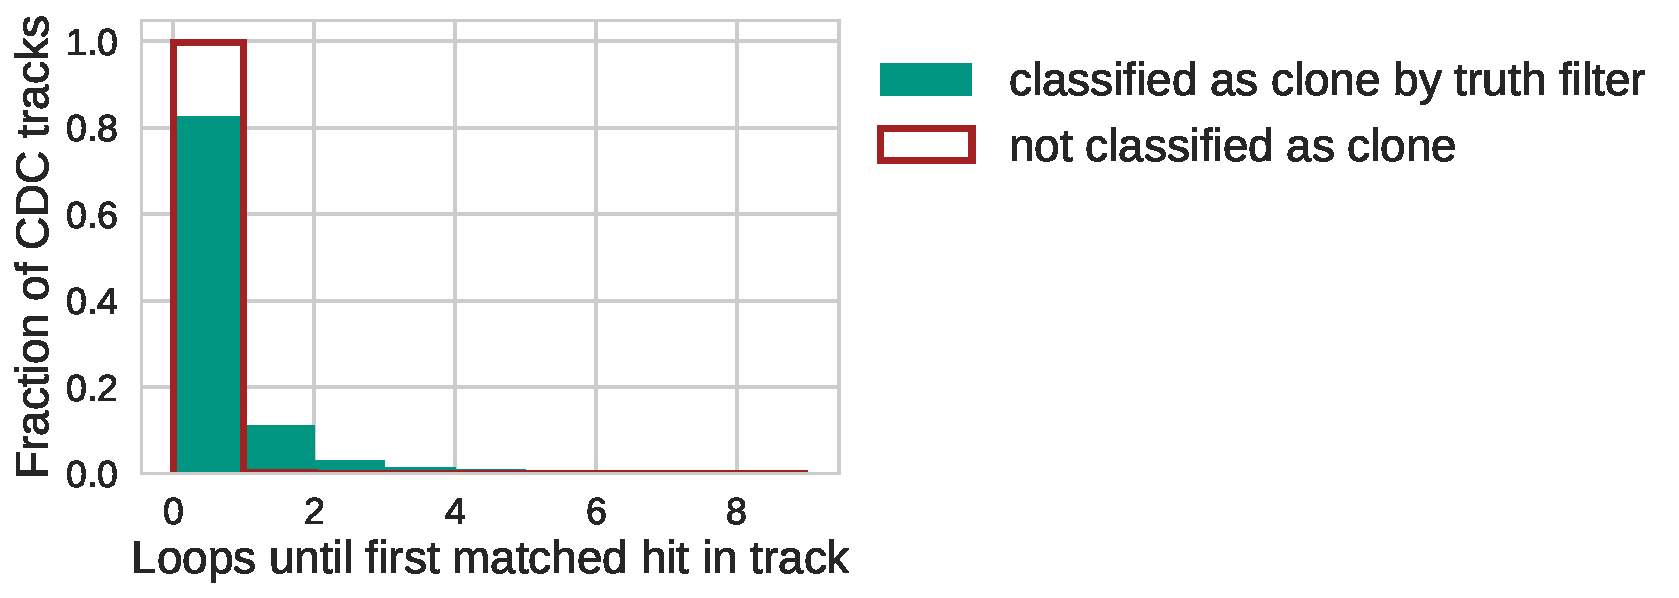
\includegraphics[width=0.7\textwidth]{figures/loop_numbers.pdf}\\
  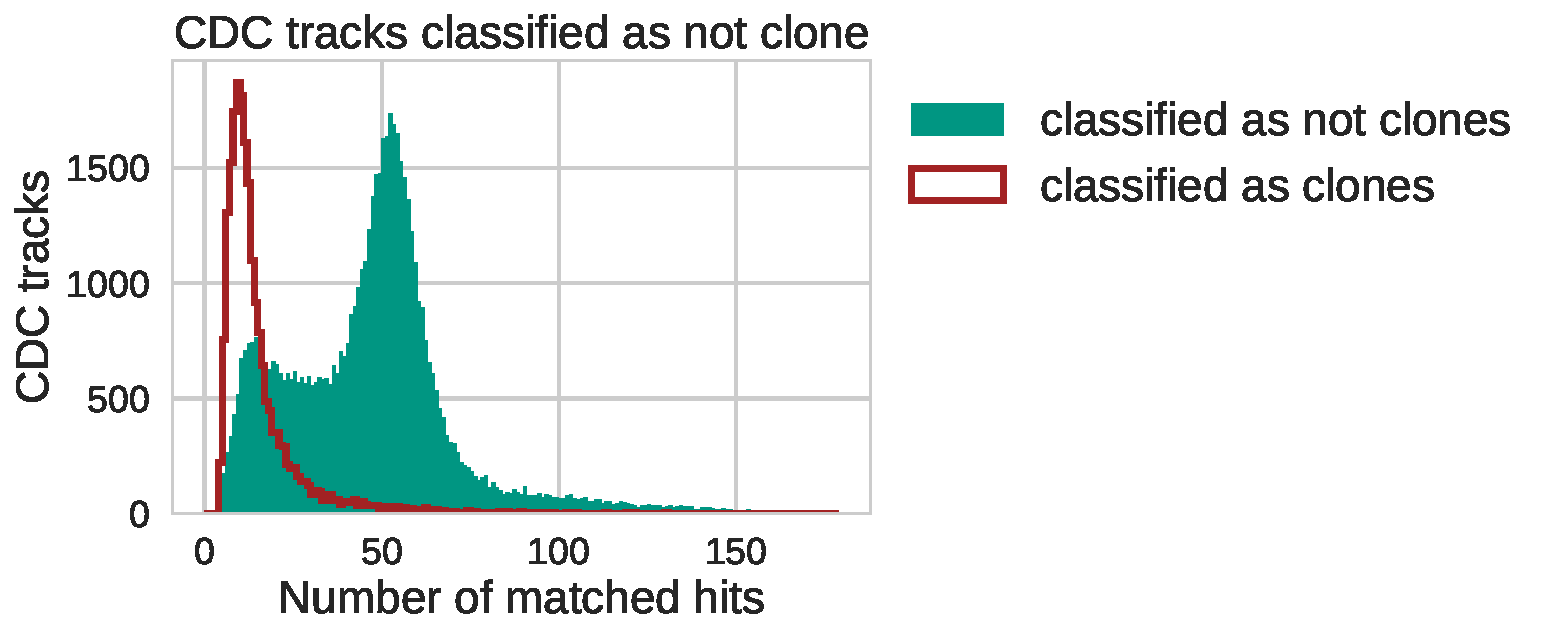
\includegraphics[width=0.7\textwidth]{figures/matched_hits.pdf}\\
\end{frame}

\end{document}

%%% Local Variables:
%%% coding: utf-8
%%% mode: LaTeX
%%% TeX-engine: default
%%% TeX-master: t
%%% ispell-dictionary: "english"
%%% synosaurus-backend: synosaurus-backend-wordnet
%%% fill-column: 100
%%% End:
%%% Local Variables: